\documentclass[a4paper,norsk, 10pt]{article}
\usepackage[utf8]{inputenc}
\usepackage{verbatim}
\usepackage{listings}
\usepackage{graphicx}
\usepackage[norsk]{babel}
\usepackage{a4wide}
\usepackage{color}
\usepackage{amsmath}
\usepackage{float}
\usepackage{amssymb}
\usepackage[dvips]{epsfig}
\usepackage[toc,page]{appendix}
\usepackage[T1]{fontenc}
\usepackage{cite} % [2,3,4] --> [2--4]
\usepackage{shadow}
\usepackage{hyperref}
\usepackage{titling}
\usepackage{marvosym }
\usepackage{subcaption}
\usepackage[noabbrev]{cleveref}
\usepackage{cite}
\usepackage{mathtools}
\usepackage{physics}


\setlength{\droptitle}{-10em}   % This is your set screw

\setcounter{tocdepth}{2}

\lstset{language=c++}
\lstset{alsolanguage=[90]Fortran}
\lstset{alsolanguage=Python}
\lstset{basicstyle=\small}
\lstset{backgroundcolor=\color{white}}
\lstset{frame=single}
\lstset{stringstyle=\ttfamily}
\lstset{keywordstyle=\color{red}\bfseries}
\lstset{commentstyle=\itshape\color{blue}}
\lstset{showspaces=false}
\lstset{showstringspaces=false}
\lstset{showtabs=false}
\lstset{breaklines}
\title{Fys3110 Hjemmeeksamen}
\author{Kadnr.: }
\begin{document}
\maketitle

\section{Exercise 1:}

\subsection{1.1)}\label{sec:11}
We have a qubit consisting of the two spin-1/2 basis states

\begin{equation}
\ket{0} \equiv \ket{\downarrow} \simeq 
\begin{pmatrix}
0 \\ 1
\end{pmatrix}
\end{equation}
\begin{equation}
\ket{1} \equiv \ket{\uparrow} \simeq 
\begin{pmatrix}
1 \\ 0
\end{pmatrix}
\end{equation}

we then introduce the operator $\hat{\sigma}_x$ represented by the Pauli-matrix

\begin{equation}
\hat{\sigma}_x \simeq
\begin{pmatrix}
0 & 1\\
1 & 0
\end{pmatrix}
\end{equation}

We can then look at how the operator acts on the basis states:

\begin{equation}
\hat{\sigma}_x\ket{0} = 
\begin{pmatrix}
0 & 1\\
1 & 0
\end{pmatrix}
\begin{pmatrix}
0 \\ 1
\end{pmatrix} = 
\begin{pmatrix}
1 \\ 0
\end{pmatrix} = \ket{1}
\end{equation}

\begin{equation}
\hat{\sigma}_x\ket{1} = 
\begin{pmatrix}
0 & 1\\
1 & 0
\end{pmatrix}
\begin{pmatrix}
1 \\ 0
\end{pmatrix} = 
\begin{pmatrix}
0 \\ 1
\end{pmatrix} = \ket{0}
\end{equation}

So the operator $\hat{\sigma}_x$ inverts the states:

\begin{equation}
\hat{\sigma}_x\ket{0} = \ket{1}, \qquad \hat{\sigma}_x\ket{1} = \ket{0}
\end{equation}

\subsection{1.2)}\label{sec:12}

We have two states $\ket{i}$ and $\ket{o}$, and the operator $G$ which acts on the states as follows:

\begin{equation}
\ket{o} = G\ket{i}, \qquad \ket{i} = G\ket{o}
\end{equation}

We can see that 

\begin{equation}
G(G\ket{o}) = G\ket{i} = \ket{o}
\end{equation}

Thus we see that $GG = I \Rightarrow G = G^{-1}$. We can check if $G$ is hermitian looking at the definition of the hermitian conjugate for some operator $K$:

\begin{equation}
\bra{\psi}K\ket{\phi} = \bra{\phi}K^\dagger\ket{\psi}^*
\end{equation}

And if $K$ is hermitian then $K = K^\dagger$ and
\begin{equation}
\bra{\psi}K\ket{\phi} = \bra{\phi}K\ket{\psi}^*
\end{equation}\label{eq:hermitDef}

We can check if this holds for $G$. For this we calculate

\begin{equation}
\bra{o}G\ket{i} = \braket{o}{o}
\end{equation}
\begin{equation}
\bra{i}G\ket{o}^* = \braket{i}{i}^* 
\end{equation}

But these qubits are normalized, so $\braket{i}{i}^*=  \braket{i}{i}=  \braket{o}{o} = 1$, and we there for get

\begin{equation}
\bra{o}G\ket{i} = 1 = \bra{i}G\ket{o}^*
\end{equation}

And thus we have used \eqref{eq:hermitDef} to show that $G$ is hermitian, $G = G^\dagger$. We have also shown that $G = G^{-1}$, but because $G$ under multiplication is a operator group, we are ensured that the identity is unique, and we an therefore conclude that $G^{-1} = G^\dagger$, which means that $G$ is unitary and hermitian.

\subsection{1.3)}

We want to find the NOT gate that switches the two states. But the operator $G$ from sec. \ref{sec:12} does exactly that: it switches $\ket{0}$ to $\ket{i}$ and vice versa. Also, we showed in sec. \ref{sec:11} that the operator $\hat{\sigma}_x$ represented as the Pauli-matrix, took a spin up to down, and down to up. We therefore know that $G$ is the operator for the NOT gate, represented by a Pauli-Matrix:

\begin{equation}
G = \hat{\sigma}_x =
\begin{pmatrix}
0 & 1\\
1 & 0
\end{pmatrix}
\end{equation}

And as shown in sec. \ref{sec:12}, this operator, $G$, is unitary hermitian.

\subsection{1.4)}
For the Hadamard gate (H-gate) we have the following operation:

\begin{equation}
H = \frac{1}{\sqrt{2}}
\begin{pmatrix}
1 & 1 \\
1 & -1
\end{pmatrix}
\end{equation}\label{eq:H}

We can look at its properties. First we find the hermitian transform of $H$:

\begin{equation}
H^\dagger = (H^T)^* = 
\frac{1}{\sqrt{2}}
\begin{pmatrix}
1 & 1 \\
1 & -1
\end{pmatrix}
= H
\end{equation}

Thus showing that $H$ is hermitian. If we multiply $H$ with it self we get

\begin{equation}
H^2 = \frac{1}{2}
\begin{pmatrix}
1 & 1 \\
1 & -1
\end{pmatrix}
\begin{pmatrix}
1 & 1 \\
1 & -1
\end{pmatrix}
=\frac{1}{2}
\begin{pmatrix}
2 & 0 \\
0 & 2
\end{pmatrix}
=
\begin{pmatrix}
1 & 0 \\
0 & 1
\end{pmatrix}
\end{equation}

This means that $H^2 = I \Rightarrow H = H^{-1}$ and that $H$ is unitary.

We can now see what $H$ does to qubit basis states

\begin{equation}
H\ket{0} = 
\frac{1}{\sqrt{2}}
\begin{pmatrix}
1 & 1 \\
1 & -1
\end{pmatrix}
\begin{pmatrix}
0 \\1
\end{pmatrix}
= \frac{1}{\sqrt{2}}
\begin{pmatrix}
1 \\ -1
\end{pmatrix}
=\frac{1}{\sqrt{2}}\left(\ket{1} - \ket{0}\right)
\end{equation}
\begin{equation}
H\ket{1} = 
\frac{1}{\sqrt{2}}
\begin{pmatrix}
1 & 1 \\
1 & -1
\end{pmatrix}
\begin{pmatrix}
1 \\ 0
\end{pmatrix}
= \frac{1}{\sqrt{2}}
\begin{pmatrix}
1 \\ 1
\end{pmatrix}
=\frac{1}{\sqrt{2}}\left(\ket{1} + \ket{0}\right)
\end{equation}


We can recognize these as the eigenstates for spin in x-direction, so

\begin{equation}
H\ket{0} = \ket{\downarrow_x}
\end{equation}\label{eq:toXdown}

\begin{equation}
H\ket{1} = \ket{\uparrow_x}
\end{equation}\label{eq:toXup}


\subsection{1.5)}
We want to find a magnetic field that that results in the effect of $H$ found is eq. \eqref{eq:toXdown} and \eqref{eq:toXup}. We look at $H$ and see that

\begin{equation}
H = \frac{1}{\sqrt{2}}\left(\sigma_x + \sigma_z\right)
\end{equation}

So we make an educated guess that the magnetic field has to we in $\hat{i} + \hat{k}$ direction. So our Hamiltonian for the magnetic field will be:

\begin{equation}
\hat{H} = -\mathbf{\mu}\cdot \mathbf{B} = - g\frac{\mu_B}{\hbar}\left(\frac{h}{\sqrt{2}}\frac{\hbar}{2}\sigma_x + \frac{h}{\sqrt{2}}\frac{\hbar}{2}\sigma_z\right) = -g\frac{h\mu_B}{2\sqrt{2}}
\begin{pmatrix}
1 & 1 \\
1 & -1
\end{pmatrix}
\end{equation}

With

\begin{equation}
\mathbf{B} = \frac{h}{\sqrt{2}}
\begin{pmatrix}
1 \\ 0 \\ 1
\end{pmatrix}
\end{equation}

The $\sqrt{2}$ being there to ensure that the magnitude of $h$. 

We now what to find the eigenstates of the Hamiltonian so we can express the time evolution of $\ket{0}$ and $\ket{1}$. This is simply done by using you favourite linear algebra program, in my case wolfram alpha:

\begin{equation}
\begin{pmatrix}
1 & 1 \\
1 & -1
\end{pmatrix}
\qquad
\rightarrow
\qquad
\ket{h_1} = 
\begin{pmatrix}
1 + \sqrt{2} \\ 1
\end{pmatrix},
\ket{h_2} = 
\begin{pmatrix}
1 - \sqrt{2} \\ 1
\end{pmatrix}
\end{equation}

with eigenvalues

\begin{equation}
h_1 = \sqrt{2},\qquad h_2  = -\sqrt{2}
\end{equation}

These eigenvectors are not normalized, but when we use them below to represent states, we get coefficients that normalizes the states. 

This gives us the energies for the Hamiltonian

\begin{equation}
E_1 = -g\frac{h\mu_B}{2}, \qquad E_2 = g\frac{h\mu_B}{2}
\end{equation}

We can now express our qubit states as linear combinations of the eigenvectors of the Hamiltonian:

\begin{equation}
\ket{1} = a\ket{h_1} + b\ket{h_2}, \qquad \ket{0} = c\ket{h_1} + d\ket{h_2}
\end{equation}

Inverting $2x2$ matrix given as $(h_1 h_2)$ we get the coefficients. This was also done with wolfram alpha:

\begin{equation}
\ket{1} = \frac{\sqrt{2}}{4}
\begin{pmatrix}
1 + \sqrt{2} \\ 1
\end{pmatrix}
-\frac{\sqrt{2}}{4}
\begin{pmatrix}
1 - \sqrt{2} \\ 1
\end{pmatrix}
\end{equation}
\begin{equation}
\ket{0} = \frac{2-\sqrt{2}}{4}
\begin{pmatrix}
1 + \sqrt{2} \\ 1
\end{pmatrix}
+\frac{2+\sqrt{2}}{4}
\begin{pmatrix}
1 - \sqrt{2} \\ 1
\end{pmatrix}
\end{equation}

We can then use the energy to add time-evolution to these states under that Hamiltonian:

\begin{equation}
\ket{1(t)} = \frac{\sqrt{2}}{4}
\begin{pmatrix}
1 + \sqrt{2} \\ 1
\end{pmatrix}
e^{iEt/\hbar}
-\frac{\sqrt{2}}{4}
\begin{pmatrix}
1 - \sqrt{2} \\ 1
\end{pmatrix}
e^{-iEt/\hbar}
\end{equation}\label{eq:upTime}
\begin{equation}
\ket{0(t)} = \frac{2-\sqrt{2}}{4}
\begin{pmatrix}
1 + \sqrt{2} \\ 1
\end{pmatrix}
e^{iEt/\hbar}
+\frac{2+\sqrt{2}}{4}
\begin{pmatrix}
1 - \sqrt{2} \\ 1
\end{pmatrix}
e^{-iEt/\hbar}
\end{equation}\label{eq:downTime}

Where $E = g\frac{h\mu_B}{2}$. We now want to find the time $t = T$ where these states have evolved into the states given by the H-gate, \eqref{eq:toXdown} and \eqref{eq:toXup}. We can do this two different ways: The first involves just comparing the components of the vectors, and then solving for $t$, but this leaves us with four equations for a single unknown. We can solve just one of these, but we want to be sure that all of the equations gives the same time $t = T$. The other way is to write these as linear combinations of $\ket{\uparrow _x}$ and $\ket{\downarrow _x}$. This will leave us with only two equations, one for $\ket{0(t)}$ and one for $\ket{1(t)}$. So lets do this. First:

\begin{equation}
\begin{pmatrix}
1 + \sqrt{2} \\ 1
\end{pmatrix}
= (1+\sqrt{2})
\begin{pmatrix}
1\\0
\end{pmatrix}
+
\begin{pmatrix}
0\\1
\end{pmatrix}
\end{equation}
\begin{equation}
=(1+\sqrt{2})
\frac{1}{2}\left[
\begin{pmatrix}
1\\1
\end{pmatrix}
+\begin{pmatrix}
1\\-1
\end{pmatrix}
\right]
+
\frac{1}{2}
\left[
\begin{pmatrix}
1\\1
\end{pmatrix}
-\begin{pmatrix}
1\\-1
\end{pmatrix}
\right]
\end{equation}


We recognize that $\begin{pmatrix} 1\\1 \end{pmatrix} = \sqrt{2}\ket{\uparrow_x}$ and $\begin{pmatrix} 1\\-1 \end{pmatrix} = \sqrt{2}\ket{\downarrow_x}$


\begin{equation}
= (1+\sqrt{2})
\frac{1}{2}\left[
\sqrt{2}\ket{\uparrow_x}
+\sqrt{2}\ket{\downarrow_x}
\right]
+
\frac{1}{2}
\left[
\sqrt{2}\ket{\uparrow_x}
-\sqrt{2}\ket{\downarrow_x}
\right]
\end{equation}
\begin{equation}
= \sqrt{2}\ket{\uparrow_x} + \ket{\uparrow_x} + \ket{\downarrow_x}
\end{equation}

And similarly

\begin{equation}
\begin{pmatrix}
1 - \sqrt{2} \\ 1
\end{pmatrix}
= \sqrt{2}\ket{\uparrow_x} - \ket{\uparrow_x} - \ket{\downarrow_x}
\end{equation}


We can now rewrite \eqref{eq:downTime} and \eqref{eq:upTime}. We start with

\begin{equation}
\ket{1(t)} = \frac{\sqrt{2}}{4}\left(\left[\sqrt{2}\ket{\uparrow_x} + \ket{\uparrow_x} + \ket{\downarrow_x}\right] e^{iEt/\hbar} - \left[\sqrt{2}\ket{\uparrow_x} - \ket{\uparrow_x} - \ket{\downarrow_x}\right]e^{-iEt/\hbar}\right)
\end{equation}
\begin{equation}
= \frac{\sqrt{2}}{4}\left(\sqrt{2}(e^{iEt/\hbar}- e^{-iEt/\hbar})\ket{\uparrow_x} + (e^{-iEt/\hbar}+ e^{iEt/\hbar})\ket{\uparrow_x} + (e^{-iEt/\hbar}+ e^{iEt/\hbar})\ket{\downarrow_x}\right)
\end{equation}
\begin{equation}
=\frac{\sqrt{2}}{4}\left(-2\sqrt{2}i\sin(Et/\hbar)\ket{\uparrow_x} + 2\cos(Et/\hbar)\ket{\uparrow_x} +2 \cos(Et/\hbar)\ket{\downarrow_x}\right)
\end{equation}

But we know that we want the to evolve into $\ket{\uparrow_x}$ as we found in \eqref{eq:toXup}. We start by finding a time where we have no $\ket{\downarrow_x}$, in other words $\cos(Et/\hbar) = 0$ This gives us the time

\begin{equation}
t = T = \frac{(2n + 1)\pi\hbar}{2E}
\end{equation}

For this time we get that the state evolves to

\begin{equation}
\ket{1(t = T)} = 
\pm i \ket{\uparrow_x}
\end{equation}\label{eq:upEvolved}

This is exactly what we wanted! But we see an extra $\pm i$, this is just an additional global phase induced by the magnetic field, and does not alter the physical state. Thus we have found the correct time for $H\ket{1}$. Now let us see if we get the same for $\ket{0}$:

\begin{equation}
\ket{0(t)} =
\frac{1}{4}\left((2-\sqrt{2})\left[\sqrt{2}\ket{\uparrow_x} + \ket{\uparrow_x} + \ket{\downarrow_x}\right] e^{iEt/\hbar} + (2+\sqrt{2})\left[\sqrt{2}\ket{\uparrow_x} - \ket{\uparrow_x} - \ket{\downarrow_x}\right]e^{-iEt/\hbar}\right)
\end{equation}

\begin{equation}
=\frac{1}{4}\bigg(2\sqrt{2}\ket{\uparrow_x}(e^{iEt/\hbar} + e^{-iEt/\hbar}) 
+ 2\ket{\uparrow_x}(e^{-iEt/\hbar} - e^{iEt/\hbar}) + 
\end{equation}
\begin{equation}
2(\ket{\uparrow_x} + \ket{\downarrow_x})(e^{iEt/\hbar} + e^{-iEt/\hbar}) 
-\sqrt{2}(\ket{\uparrow_x} + \ket{\downarrow_x})(e^{iEt/\hbar} + e^{-iEt/\hbar}) 
\bigg)
\end{equation}

\begin{equation}
= \frac{1}{4}\left(4\sqrt{2}\cos(Et/\hbar) + 4i\sin(Et/\hbar)\ket{\downarrow_x} - 2\sqrt{2}(\ket{\uparrow_x} + \ket{\downarrow_x})\cos(Et/\hbar)\right)
\end{equation}

Again we known hat we what the state to evolve to, namely $\ket{\downarrow_x}$ \eqref{eq:toXdown}. So we need to remove all $\ket{\uparrow_x}$. Fortunately, like last time, this can be done be letting $\cos(Et/\hbar) = 0$. This is true for 

\begin{equation}
t = T = \frac{(2n + 1)\pi\hbar}{2E}
\end{equation}

Just like for $\ket{1(t)}$. We then get

\begin{equation}
\ket{0(t=T)} = \pm i \ket{\downarrow_x}
\end{equation}\label{eq:downEvolved}

Here again we see the same global phase, and since it doesn't change the physical state, the state has evolved as desired, and we have found the correct time.

We got the same time for both $\ket{0(t)}$ and $\ket{1(t)}$.

\begin{equation}
T = \frac{(2n + 1)\pi\hbar}{2E}
\end{equation}

Since we can chose the integer $n$ the simplest thing is to set it to $0$. So in summary:


To implement the H-gate we can send the qubit through a magnetic field of strength $h$ pointed in the $\frac{h}{\sqrt{2}}(\hat{i} + \hat{k})$ direction. The magnetic field is turned on at $t = 0$ and turned off at 

\begin{equation}
t  = T = \frac{\pi\hbar}{2E} = \frac{\pi \hbar}{g h \mu_B} = \frac{2m \pi}{g h e}
\end{equation}

\section{Exercise 2:}

\subsection{2.1)}\label{sec:21}

We have a boolean function

\begin{equation}
f(i)=
\begin{cases}
True, & i = i^* \\
False, & i \neq i^*
\end{cases}
\end{equation}

If we have a set of values $i = \{1,\ldots, N\}$. We will for large $N$ use $n = \frac{N}{2}$ applications of $f$ on average to find $i = i^*$. This is contingent on that the probability of guessing correct is always $1/N$. In that case

\begin{equation}
\langle n \rangle = \sum_n nP(n) = \sum_n n \frac{1}{N} = \frac{1}{N}\sum_n n = \frac{N+1}{2} \approx \frac{N}{2}
\end{equation}

There may be some approximations in this calculations, but it is intuitive that the average number of applications are on the order of $N$.

\subsection{2.2)}

We have the operators which works like

\begin{equation}
F\ket{i} = 
\begin{cases}
-\ket{i^*} & , i = i^* \\
\ket{i} & , i \neq i^*
\end{cases}
\end{equation}\label{eq:Feffect}

We want to show that $F$ can be written as

\begin{equation}
F = I - 2\ket{i^*}\bra{i^*}
\end{equation}\label{eq:Foperator}

Let's use the operator on a ket

\begin{equation}
F\ket{i} = (I - 2\ket{i^*}\bra{i^*})\ket{i} = I\ket{i} - 2\ket{i^*}\bra{i^*}\ket{i}
\end{equation}

\begin{equation}
= \ket{i} - 2\delta_{i,i^*}\ket{i^*} =
\begin{cases}
-\ket{i^*} & , i = i^* \\
\ket{i} & , i \neq i^*
\end{cases}
\end{equation}

We can see that this gives the same as \eqref{eq:Feffect}, and we can therefore write $F = I - 2\ket{i^*}\bra{i^*}$.

We can see from eq. \ref{eq:Foperator} that $F$ is a Householder transformation, which ensures that $F$ is unitary hermitian, but we can also show this:

\begin{equation}
F(F\ket{i}) = (I - 2\ket{i^*}\bra{i^*})(I - 2\ket{i^*}\bra{i^*})\ket{i}
\end{equation}
\begin{equation}
= I\ket{i} - 2\ket{i^*}\bra{i^*}I\ket{i} -2I\ket{i^*}\bra{i^*}\ket{i} + 4\ket{i^*}\bra{i^*}\ket{i^*}\bra{i^*}\ket{i}
\end{equation}
\begin{equation}
= \ket{i} - 4\ket{i^*}\bra{i^*}\ket{i} + 4\ket{i^*}\bra{i^*}\ket{i} = \ket{i}
\end{equation}

Thus $FF = I \Rightarrow F = F^{-1}$. We then show that $F$ is hermitian:

\begin{equation}
F^\dagger = (I - 2\ket{i^*}\bra{i^*})^\dagger = I - 2(\ket{i^*}\bra{i^*})^\dagger
\end{equation}
\begin{equation}
= I - 2(\bra{i^*})^\dagger(\ket{i^*})^\dagger = I - 2\ket{i^*}\bra{i^*} = F
\end{equation}

So $F$ is hermitian, $F = F^\dagger$. This implies that $F$ is unitary hermitian:

\begin{equation}
F^{-1} = F = F^\dagger \Leftrightarrow F^\dagger = F^{-1}
\end{equation}


\subsection{2.3}
We now introduce the superposition of the states $\ket{i}$

\begin{equation}
\ket{s} = \frac{1}{\sqrt{N}} \sum_{i=1}^N \ket{i}
\end{equation}

We then calculate 

\begin{equation}
\braket{i^*}{s} = \frac{1}{\sqrt{N}} \sum_{i=1}^N \braket{i^*}{i} = \frac{1}{\sqrt{N}} \sum_{i=1}^N \delta_{i,i^*} = \frac{1}{\sqrt{N}} 
\end{equation}\label{eq:is}


and

\begin{equation}
F\ket{s} = I\ket{s} - 2\ket{i^*}\bra{i^*}\ket{s} = \ket{s} - \frac{2}{\sqrt{N}}\ket{i^*}
\end{equation}\label{eq:Fs}



\subsection{2.4)}

We now consider the state:

\begin{equation}
\ket{g} = \alpha \ket{s} + \beta\ket{i^*}
\end{equation}

We want this to be normalized:

\begin{equation}
\braket{g}{g} = 1
\end{equation}

Due to Riesz representation theorem, we know that such a bra $\bra{g}$ exist, so we can then find the condition for $\alpha$ and $\beta$ such that $\ket{g}$ is normalized.

\begin{equation}
(\alpha* \bra{s} + \beta*\bra{i^*})(\alpha \ket{s} + \beta\ket{i^*}) = |\alpha|^2 + |\beta|^2 + \alpha\beta* \braket{s}{i^*} + \alpha*\beta \braket{i^*}{s}
\end{equation}

$\alpha$ and $\beta$ are both real. We know that $\braket{i^*}{s}$ is real from \eqref{eq:is}, so $\braket{s}{i^*} = \braket{i^*}{s}* = \braket{i^*}{s}$. So: 

\begin{equation}
\alpha^2 + \beta^2 + \frac{2\alpha \beta}{\sqrt{N}} = 1
\end{equation}\label{eq:conditionAB}

Is the condition that makes sure that $\ket{g}$ is normalized.

\subsection{2.5)}

The operator for measuring the measurement $i$ of state $\ket{i}$ is named $X$, so $X$ acting on a state $\ket{i}$ is:

\begin{equation}
X\ket{i} = i\ket{i}
\end{equation}

meaning that $\ket{i}$ are eigenstates of $X$ with eigenvalue $i$. This means that we can use the spectral theorem to write $X$ as a spectral representation with $\ket{i}$ and $i$:

\begin{equation}
X = \sum_{j=1}^N j\ket{j}\bra{j}
\end{equation}

($j$ and $i$ are dummy indices and therefore interchanged).

\subsection{2.6)}

We want to find the probability of measuring $i^*$ when observing $\ket{g}$. From $X$ we find

\begin{equation}
X\ket{i^*} =\sum_{j=1}^N j\ket{j}\bra{j}\ket{i^*} = \sum_{j=1}^N j\ket{j}\delta_{j,i^*} = i^*\ket{i^*} 
\end{equation}

Meaning that $\ket{i^*}$ is the state where we measure $i^*$, meaning that we need to find the probability of measuring $\ket{g}$ in state $\ket{i^*}$. We d this with the projection operator

\begin{equation}
\hat{P} = \ketbra{i^*}{i^*}
\end{equation}

We then find the expectation value of $P$ acting on $\ket{g}$:

\begin{equation}
P(i^*) = \bra{g}\hat{P}\ket{g} = \bra{g}\ket{i^*}\bra{i^*}\ket{g} = |\braket{i^*}{g}|^2
\end{equation}

We can calculate this

\begin{equation}
\braket{i^*}{g} = \bra{i^*}(\alpha \ket{s} + \beta\ket{i^*}) = \alpha\braket{i^*}{s}+ \beta \braket{i^*}{i^*} = \frac{\alpha}{\sqrt{N}} + \beta
\end{equation}

All the terms are real, so the norm in the probability just becomes a power of two:

\begin{equation}
\Rightarrow P(i^*) = |\braket{i^*}{g}|^2 = \left(\frac{\alpha}{\sqrt{N}} + \beta\right)^2 = \frac{\alpha^2}{N} + \beta^2 + \frac{\alpha\beta}{\sqrt{N}}
\end{equation}

From eq. \eqref{eq:conditionAB} we see that

\begin{equation}
\beta^2 + \frac{2\alpha \beta}{\sqrt{N}}  = 1 - \alpha^2
\end{equation}

So we get that the probability of measuring $i^*$ becomes:

\begin{equation}
P(i^*) = 1 - \alpha^2\left(1 - \frac{1}{N}\right)
\end{equation}\label{eq:prob}

\subsection{2.7)}

We now introduce the operator

\begin{equation}
U = 2\ketbra{s}{s} - I
\end{equation}\label{eq:U}

We want to look at $UF\ket{s}$. We already calculated $F\ket{s}$\eqref{eq:Fs}, so we get: 

\begin{equation}
UF\ket{s} = U(\ket{s} - \frac{2}{\sqrt{N}}\ket{i^*})
\end{equation}
\begin{equation}
= 2\ket{s}\braket{s}{s} - I\ket{s} - \frac{4}{\sqrt{N}}\ket{s}\braket{s}{i^*} + \frac{2}{\sqrt{N}}I\ket{i^*} = \ket{s} - \frac{4}{N}\ket{s} + \frac{2}{\sqrt{N}}\ket{i^*} 
\end{equation}

So

\begin{equation}
UF\ket{s} =  \left(1 - \frac{4}{N}\right)\ket{s} + \frac{2}{\sqrt{N}}\ket{i^*} 
\end{equation}\label{eq:UFs}


If we look at $U$\eqref{eq:U} we see that it too is a Householder transformation(with a negative sign), thus we know that it is unitary hermitian. A unitary always preserves the norm. So if we first apply $F$(which we showed was unitary) to $\ket{s}$, its norm is still $1$ ($\ket{s}$ is a normalized sum of normalized states). So when we then apply $U$, the norm is still $1$. Thus the norm of $UF\ket{s}$ is $1$. But we can also show this explicit:

\begin{equation}
\left[\left(1 - \frac{4}{N}\right)\bra{s} + \frac{2}{\sqrt{N}}\bra{i^*}\right]\left[\left(1 - \frac{4}{N}\right)\ket{s} + \frac{2}{\sqrt{N}}\ket{i^*}\right]
\end{equation}

(remember that all the constants are real)

\begin{equation}
= \left(1 - \frac{4}{N}\right)^2\braket{s}{s} +\frac{2}{\sqrt{N}} \left(1 - \frac{4}{N}\right)\bra{s}\ket{i^*} + \frac{2}{\sqrt{N}} \left(1 - \frac{4}{N}\right)\bra{i^*}\ket{s} + \frac{4}{N}\braket{i^*}{i^*}
\end{equation}

\begin{equation}
= \left(1 - \frac{4}{N}\right)^2 + \frac{4}{N}\left(1 - \frac{4}{N}\right) + \frac{4}{N}
\end{equation}
\begin{equation}
= 1 - \frac{8}{N} + \frac{16}{N^2} + \frac{4}{N} - \frac{16}{N^2} + \frac{4}{N} = 1
\end{equation}


So we have showed that the norm of $UF\ket{s}$ is $1$.


\subsection{2.8)}

We now want to calculate $UF\ket{g}$:

\begin{equation}
UF\ket{g} = UF(\alpha\ket{s} + \beta\ket{i^*}) = \alpha UF\ket{s} + \beta UF\ket{i^*}
\end{equation}

We have already found $UF\ket{s}$\eqref{eq:UFs}, but we need to find

\begin{equation}
UF\ket{i^*} = -U\ket{i^*} = -(2\ketbra{s}{s} - I)\ket{i^*} = -2\ket{s}\braket{s}{i^*} + I\ket{i^*}
\end{equation}
\begin{equation}
= \ket{i^*} - \frac{2}{\sqrt{N}}\ket{s}
\end{equation}


We can now combine these

\begin{equation}
\alpha UF\ket{s} + \beta UF\ket{i^*} = \alpha\left[\left(1 - \frac{4}{N}\right)\ket{s} + \frac{2}{\sqrt{N}}\ket{i^*} \right] + \beta\left[\ket{i^*} - \frac{2}{\sqrt{N}}\ket{s}\right]
\end{equation}

We can so sort these and find 

\begin{equation}
UF(\alpha\ket{s} + \beta\ket{i^*}) = \left[\alpha\left(1 - \frac{4}{N}\right) - \frac{2\beta}{\sqrt{N}}\right]\ket{s} + \left[\frac{2\alpha}{\sqrt{N}} + \beta\right]\ket{i^*}
\end{equation}\label{eq:UFg}

\subsection{2.9)}

We can numerically compute the probability of measuring $i^*$ in the state $(UF)^n\ket{s}$. But as we can see from eq. \eqref{eq:UFs} we get a contribution from $\ket{i^*}$, and it gets the same form as $UF\ket{g}$, thus this is the same as calculating $(UF)^n\ket{g}$ with the initial conditions $\beta = 0$. We know from eq. \ref{eq:UFg} how this system evolve. We can write the coefficients in front of $\ket{s}$ and $\ket{i^*}$ as $\alpha_{new}$ and $\beta_{new}$ and get a simple algorithm for calculating evolution under $UF$\eqref{item:algo}. Each time we update the system we check the probability of measuring $i^*$ we found in \eqref{eq:prob}.

We want to find for what $n$ we get $99\%$ of measuring $i^*$. To do this we simply exit the loop when this probability is reached, saving the $n$ at which this happens.

The final algorithm looks like this:

\begin{itemize}\label{item:algo}
\item Start with $\alpha = 1$, $\beta = 0$
\item loop over n:
\subitem Calculate $\alpha_{new} = \left[\alpha\left(1 - \frac{4}{N}\right) - \frac{2\beta}{\sqrt{N}}\right]$ and $\beta_{new} = \left[\frac{2\alpha}{\sqrt{N}} + \beta\right]$
\subitem Set $\alpha = \alpha_{new}$ and $\beta = \beta_{new}$
\subitem Find the probability $P(i^*) = 1 - \alpha^2\left(1 - \frac{1}{N}\right)$
\subitem If $P(i^*) \geq 0.99$:
\subsubitem Save n
\subsubitem Exit loop
\end{itemize}

The code is found at the end\ref{sec:code}.


If we don't exit the loop after $P \neq 0.99$ but look at how the probability evolves:

\begin{figure}[H]
    \centering
    \begin{subfigure}[b]{0.3\textwidth}
        \includegraphics[width=\textwidth]{P1e3.png}
        \caption{Probability for $N = 10^3$}
        \label{fig:P1e3}
    \end{subfigure}
    ~ %add desired spacing between images, e. g. ~, \quad, \qquad, \hfill etc. 
      %(or a blank line to force the subfigure onto a new line)
    \begin{subfigure}[b]{0.3\textwidth}
        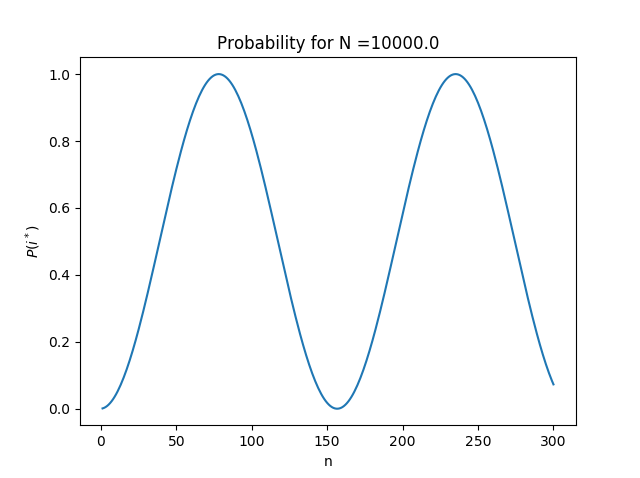
\includegraphics[width=\textwidth]{P1e4.png}
        \caption{Probability for $N = 10^4$}
        \label{fig:P1e4}
    \end{subfigure}
    ~ %add desired spacing between images, e. g. ~, \quad, \qquad, \hfill etc. 
    %(or a blank line to force the subfigure onto a new line)
    \begin{subfigure}[b]{0.3\textwidth}
        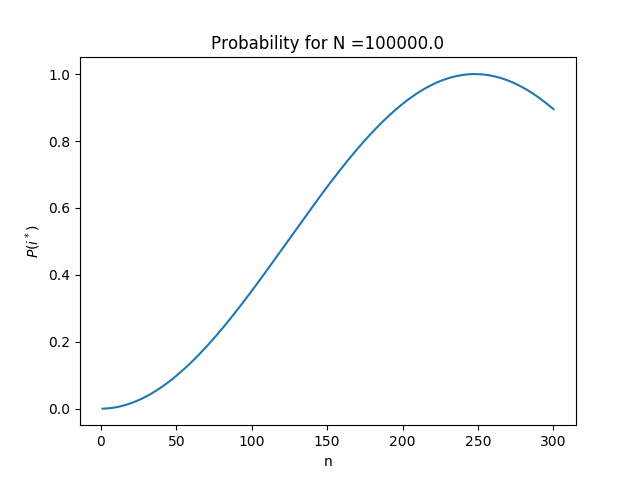
\includegraphics[width=\textwidth]{P1e5.png}
        \caption{Probability for $N = 10^5$}
        \label{fig:P1e5}
    \end{subfigure}
    \caption{We can see that the probability of measuring $i^*$ actually goes as a sinusoidal function of $n$. This means that using $UF$ doesn't always imporove the probability, and that there are regoins where applying $UF$ actually lowers the probability. We also see that frequancy of this sinusoidal function increases with the number of unknown states $N$, and thus we need to apply $UF$ more times to get a better probability.}\label{fig:prob}
\end{figure}


We can then look at how many $n = n^*$ is necessary to get a probability $P(i^*)\geq 0.99$:

\begin{table}[H]
\centering
\begin{tabular}{c | c}
$N$ & $n*$\\
\hline 
$10^3$ & $23$\\
$10^4$ & $74$\\
$10^5$ & $233$
\end{tabular}
\caption{A table showing the many times $UF$ is applied, $n^*$, to get a probability $\geq 99\%$ to measure $i^*$.}
\end{table}

To see a clearer pattern we use $800$ points, and plots the result:

\begin{figure}[H]
\centering
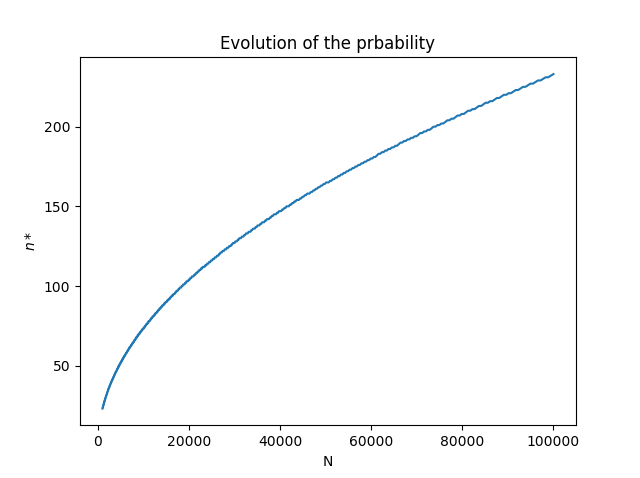
\includegraphics[scale=0.5]{pi.png}
\caption{The number of times $n^*$ we need to apply $UF$ to get a probability $P(i^*)\geq 0.99$ }
\end{figure}



We can see that as $N$ increases, so does the number if times we need to apply $UF$ this number $n^*$. It looks quite like a square root, but we need to make sure. For this we use a log-log plot, this is because:

\begin{equation}
n^* = N^i \Rightarrow \log(n^*) = i\cdot \log(N)
\end{equation}

So we can use the log-log plot, find the slope and therefore find the order of N of which $n^*$ increases.


\begin{figure}[H]
\centering
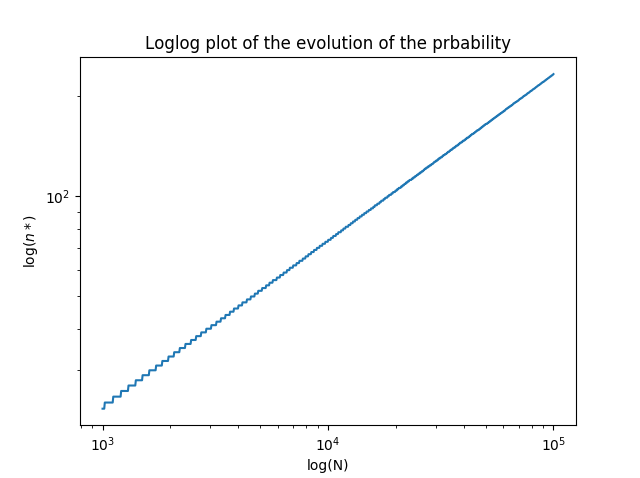
\includegraphics[scale=0.5]{logpi.png}
\caption{This shows $\log(n^*)$ vs $\log(n)$ and clearly shows a straight line. The slope of this line is the order of $N$ at which $n^*$ increases.}
\end{figure}


If we use a normal finite difference on this curve(which is exact for a linear function), we find that slope is $\sim 0.503$. This is close enough to $1/2$ that we can conclude that

\begin{equation}
n^* \sim O(\sqrt{N})
\end{equation}

This is an immense improvement over the classical result from sec. \ref{sec:21}, but more on this below.


\subsection{2.10)}
As shown in sec. \ref{sec:21} a classical algorithm for finding a member $i^*$ of a set scales like $O(N)$.

We can instead use quantum mechanics. We can then make the set of values to a set of states $\ket{i}$. We then make a equal amplitude superposition state $\ket{s}$ of these states $\ket{i}$. We then apply the operator $UF$ to $\ket{s}$ we will get a state which is a superposition $\ket{s}$ and our target state $\ket{i^*}$, namely $\ket{g}$. We can then calculate the probability of measuring $\ket{g}$ in state $\ket{i^*}$. If this probability is to low, we apply $UF$ again. This makes a new superposition of $\ket{s}$ and $\ket{i^*}$(still $\ket{g}$ but with new coefficients) \ref{eq:UFg}. This is done until the desired probability is reached, $99\%$ in our case. When this probability is reached we can measure the system, and get the value $i^*$. This is called a 'Grover iteration'(more on this below).

This is a quantum algorithm used in a quantum computer. And as we saw in the section above it manage to find $i^*$ with in a time that scales like $O(\sqrt{N})$. This is an immense improvement over the classical algorithm, and is the reason quantum computers are the future!

\subsubsection{Testing}
\textit{This section is far beyond what is asked for, and is more for the fun of it, but illustrates the efficiency of the quantum computer!}

The above algorithm is called Grovers algorithm. It is simple to implement on a real quantum processor, and can be done with only 3 quantum gates: the well known Hadamard gate, the Pauli X-gate and a controlled-NOT gate. Schematically this is the setup:

\begin{figure}[H]
\centering
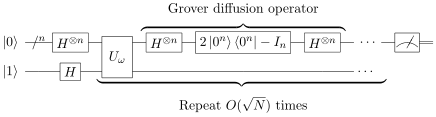
\includegraphics[scale=0.5]{grover.png}
\caption{Schematic drawing of the Grover algorithm. Taken from \emph{REF}}
\end{figure}

Finding this interesting I tried running this on the IBM ibmqx4 5 qubit processor. Due to the limited size of the processor I could only use $N=4$. But it is still impressive. Lets find how many iterations we need of $UF$. From \eqref{eq:UFg} we get (by starting with $\alpha = 1$, $\beta = 0$)

\begin{equation}
\alpha_{new} = \left[\left(1 - \frac{4}{N}\right) - \frac{2\cdot 0}{\sqrt{N}}\right] = 0, \qquad \beta_{new} = \left[\frac{2}{\sqrt{4}} + 0\right] = 1
\end{equation}

This means that only after one(!) use of $UF$ we get a probability of measuring $i^*$:

\begin{equation}
P(i^*) = 1 - \alpha^2_{new}\left(1 - \frac{1}{N}\right) = 1
\end{equation}

So we should 'guess' correct every time, which is incredible!

So lets do this in reality. I implemented the algorithm on the ibmqx4 with the help of IBMs own tutorials(I'm not smart enough to do this by myself yet)\emph{REF}. Schematically it becomes:

\begin{figure}[H]
\centering
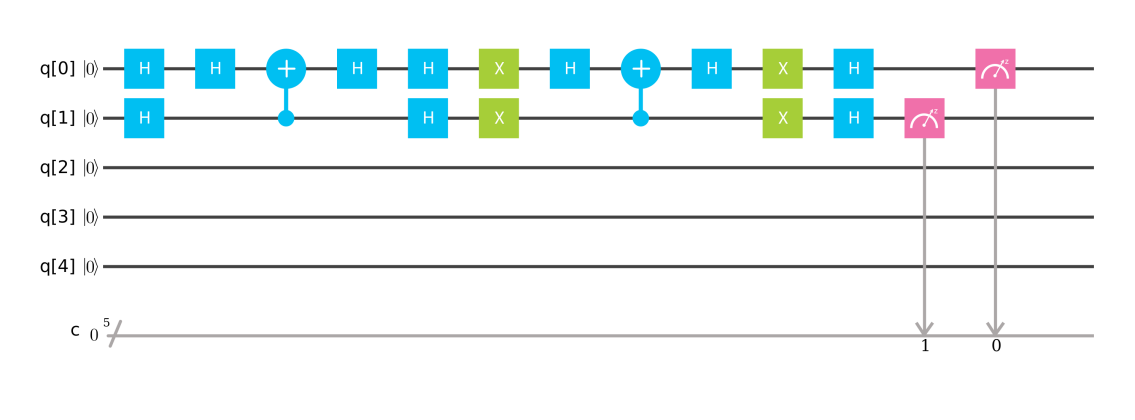
\includegraphics[scale=0.2]{groverIBM.png}
\caption{Schematic drawing of the Grover algorithm as used on ibmqx4 processor.}
\end{figure}

Fist $i^*$ is placed at qubit $00011$ (this is of course unknown to the system), this is done by gate 2-4. $UF$ is applied once, gate 5-11. The result is then measured. The result is as follows:

\begin{figure}[H]
\centering
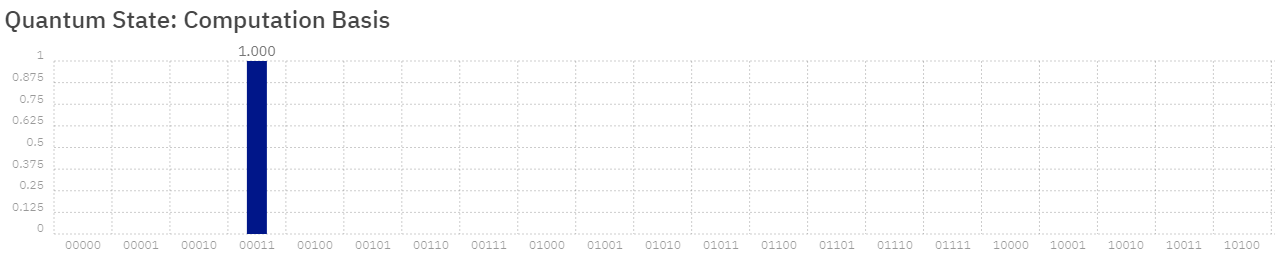
\includegraphics[scale=0.4]{IBMresultat.png}
\caption{The results form the ibmqx4 processor, showing that the quantum processor quest correctly.}
\end{figure}

As we can see the the processor measured that $i^*$ should be at $00011$, which is correct. Meaning that the quantum computer managed to guess the correct $i^*$ when 'guessing' on four possible values on the first try!  This is just as the theory expected!

This was totally unnecessary according to the exercise, but is a nice illustration of the power of the quantum computer. It is also incredible that IBM lest the public use there quantum processor, so this was a chance I could not let walk me by.
\section{Code}\label{sec:code}
\lstinputlisting{29.py}


\end{document}

